\documentclass[11pt]{amsart}
\usepackage[T1]{fontenc}
\usepackage{lmodern,microtype,amsmath,amssymb,mathtools,booktabs,array,enumitem}
\usepackage{longtable,needspace}
\usepackage{tikz,listings}
\usetikzlibrary{arrows.meta,positioning}
\lstset{basicstyle=\ttfamily\small,breaklines=true,columns=fullflexible,
 keepspaces=true,showstringspaces=false,escapeinside={(*@}{@*)}}
\usepackage[hidelinks]{hyperref}
\usepackage[nameinlink,noabbrev]{cleveref}
\urlstyle{same}
\hypersetup{pdftitle={Erd\H{o}s--Szekeres: Upper Bounds for Convex Heptagons and Octagons},pdfauthor={Michael Schroeder},pdfsubject={Erdos-Szekeres bounds with Lean formalization},pdfkeywords={Erd\H{o}s--Szekeres problem, convex polygons, cups and caps}}
\allowdisplaybreaks[2]
\numberwithin{equation}{section}
\newtheorem{theorem}{Theorem}[section]
\newtheorem{proposition}[theorem]{Proposition}
\newtheorem{lemma}[theorem]{Lemma}
\newtheorem{corollary}[theorem]{Corollary}
\theoremstyle{definition}
\newtheorem{definition}[theorem]{Definition}
\theoremstyle{remark}
\newtheorem{remark}[theorem]{Remark}
\DeclareMathOperator{\ES}{ES}
\DeclareMathOperator{\conv}{conv}
\newcommand{\set}[1]{\{#1\}}
\newcommand{\down}{\mathord{\downarrow}}
\newcommand{\cupS}{S_{\cup}}
\newcommand{\capS}{S_{\cap}}
\newcommand{\cupE}{E_{\cup}}
\newcommand{\capE}{E_{\cap}}
\newcommand{\code}[1]{\texttt{\small #1}}
\title[Convex heptagons and octagons]{Erd\H{o}s--Szekeres: Upper Bounds for Convex Heptagons and Octagons}
\author{Michael Schroeder}
\address{Independent Researcher}
\thanks{ORCID: \href{https://orcid.org/0009-0004-3249-0195}{0009-0004-3249-0195}. Version 1, 19 September 2026.\newline\mbox{DOI: \href{https://doi.org/10.5281/zenodo.22842891}{10.5281/zenodo.22842891}}.}
\subjclass[2020]{Primary 52C10; Secondary 05D10, 68V15}
\keywords{Erd\H{o}s--Szekeres problem, convex polygons, cups and caps}
\date{19 September 2026}
\begin{document}
\begin{abstract}
The Erd\H{o}s--Szekeres number $\ES(n)$ is the least $N$ such that
every set of $N$ points in the plane, with no three collinear, contains
$n$ points in convex position. We prove $\ES(7)\le81$ and
$\ES(8)\le319$. Both bounds follow from a common geometric partition
and exact finite certificates for the resulting cup--cap configurations.
The heptagon proof combines a five-point transversal with exclusions
that preserve shared geometric witnesses. The octagon proof counts
missing Ferrers states using hereditary convexity and four-cap compression.
We also establish the $(7,5,6)$ case of the Erd\H{o}s--Tuza--Valtr
conjecture: the largest planar set in general position with distinct
abscissae avoiding a convex heptagon, a five-cap, and a six-cup has
25 points. All three upper bounds are formalized in Lean,
including the geometric reductions and the validity of the finite
encodings. The accompanying archive provides sources, exact certificates,
and independent checkers. Finite Lean checks use native evaluation
with an explicitly documented trust boundary.
\end{abstract}
\maketitle
\raggedbottom

\section{Introduction}
Let $\ES(n)$ denote the least integer $N$ such that every set of at least
$N$ points in $\mathbb R^2$, with no three collinear, contains $n$ points
in convex position. The polygon need not be empty. Erd\H{o}s and
Szekeres~\cite{ES35,ES61} proved
\[
 2^{n-2}+1\le\ES(n)\le\binom{2n-4}{n-2}+1
\]
and conjectured equality with the lower bound. Szekeres and
Peters~\cite{SP} established $\ES(6)=17$ by a computer proof.
The next two conjectured values are $33$ and $65$.

\begin{theorem}\label{thm:main}
Every set of $81$ points in the plane in general position contains a
convex heptagon, and every such set of $319$ points contains a convex
octagon. Consequently,
\[
 33\le\ES(7)\le81,\qquad 65\le\ES(8)\le319.
\]
\end{theorem}

Our contribution is a finite strengthening of the cup--cap method,
with a complete formal connection to planar geometry. We use the
classical projective reduction, a residual partition, and injective
encodings by Ferrers down-sets. The heptagon proof rules out a balanced
fifty-point equality case while keeping one shared system of actual
witnesses. The octagon proof uses a different certificate: weighted
omission inequalities on small families whose occupied states force
convexity. Both arguments retain every chronological order allowed by
their necessary constraints.

Here is the numerical structure. Write $M_n(a,b)$ for the maximum size
of a set avoiding a convex $n$-gon, an $a$-cap, and a $b$-cup, in that
parameter order. Put $C_n=M_n(n-1,n-1)$, and let $D_n$ be the maximum
size of a set containing no $(n-2)$-cap, no convex $n$-gon, and no point
simultaneously ending an $(n-2)$-cup and starting an $(n-3)$-cap.
Both witnesses in the last condition must lie in the same set.
Sections~\ref{sec:geometry}--\ref{sec:partition} prove
\begin{equation}\label{eq:bridge}
 \ES(n)\le C_n+D_n+2\qquad(n\ge6).
\end{equation}
The savings in the two avoiding maxima are as follows.
\begin{center}
\begin{tabular}{crrrrr}
\toprule
$n$ & $C_n$: baseline & here & $D_n$: baseline & here & Total saving\\
\midrule
7 & 70 & 49 & 41 & 30 & $21+11=32$\\
8 & 252 & 193 & 154 & 124 & $59+30=89$\\
\bottomrule
\end{tabular}
\end{center}
All entries are upper bounds. Before imposing polygon-capacity rows,
the cup--cap count gives $\binom{2n-6}{n-3}$ balanced states.
The two-sided residual construction in Section~\ref{sec:319} gives
$\binom{2n-6}{n-4}-\binom{2n-8}{n-5}$ states: in the
$(n-4)\times(n-2)$ rectangle, the forbidden junction excludes the
maximal cell $(1,n-2)$. At $n=7,8$ these give respectively
$70+41+2=113$ and $252+154+2=408$.
The two-point adjustment includes one deleted projective root and the
conversion from an avoiding maximum to a forcing threshold.

We also prove the sharp restricted equality $M_7(5,6)=25$
(Theorem~\ref{lem:B25}), a case of the conjecture of
Erd\H{o}s, Tuza, and Valtr~\cite{ETV}. The conjectured value is
$\sum_{i=1}^{3}\binom5i$. Baek--Balko~\cite[Section~2.1]{BB}
record the previously known cases as $n\ge a+b-3$ or $a=4$ or $b=4$;
$(n,a,b)=(7,5,6)$ lies outside these ranges. The lower construction is
classical~\cite{ES61,ETV}; the upper bound is the new certificate.
Reflection gives the mirrored case $(7,6,5)$.

\subsection{Previous work}
T\'oth and Valtr's projective method~\cite{TV98,TV05} underlies the
reduction used below. The explicit finite bound of Nassajian Mojarrad
and Vlachos~\cite[Theorem~1.1]{MV} is
\begin{equation}\label{eq:MV}
 \ES(n)\le\binom{2n-5}{n-2}-\binom{2n-8}{n-3}+2\qquad(n\ge6),
\end{equation}
which gives $113$ and $408$. Our bounds improve these by $32$ and $89$,
respectively. Norin and Yuditsky~\cite{NY} obtain the asymptotic factor
$7/8$ by encoding incoming and outgoing chains. Their three-chain
argument is used in our residual partition. Suk~\cite{Suk} proves
$\ES(n)=2^{n+o(n)}$; Holmsen, Nassajian Mojarrad, Pach and
Tardos~\cite{HMPT} refine the upper bound to
$2^{n+O(\sqrt{n\log n})}$. These asymptotic expressions do not by
themselves supply explicit improvements at $n=7,8$.

The strong- and weak-polygon analogues of the Erd\H{o}s--Szekeres
conjecture fail for arbitrary red--blue colorings of ordered triples
already at $k=7$: Balko--Valtr~\cite{BV} prove $C_{\mathrm{strong}}(7)>33$,
and Baek--Balko~\cite{BB} prove $C_{\mathrm{weak}}(7)>33$.
Here $C_{\mathrm{strong}}$ and $C_{\mathrm{weak}}$ are the corresponding
forcing thresholds. A weak $k$-gon consists of differently colored
monotone paths with common endpoints and vertex counts summing to
$k+2$; a strong $k$-gon additionally requires disjoint interiors.
The signotope extension remains open: Baek--Balko
\cite[Section~3]{BB} relate it to the Goodman--Pollack conjecture.
Our results concern real planar sets; a signotope interpretation of
the complete proof has not been audited.
Down-set encodings of ordered paths are established machinery
\cite{MS}. Baek~\cite{Baek} proves that
$\binom{n-1}{2}+2$ points force a four-cap or a convex $n$-gon;
its $n=8$ case is a numerical input to our block-compression argument.
Baek and Balko~\cite{BB} obtain sharp split-polygon thresholds and
results for decomposable configurations. A split polygon permits
unmatched left endpoints, so its threshold cannot be substituted for
the unrestricted convex-polygon threshold.

Recent computational work also emphasizes the distinction between an
encoding and a complete exclusion. Dumitru~\cite{Dumitru} reports
refutations of anchored thirty-three-point subfamilies, without an
exhaustive cover. Dam\'asdi, Dong, Scheucher and Zeng~\cite{DDSZ} construct
small saturated sets, showing why failure to extend one example need
not establish a maximum. Koshelev and Koshka~\cite{KK} develop SAT/ASP
models and fixed-abscissa realization searches for related variants.
Infeasibility with fixed abscissae does not exclude arbitrary coordinates.
None of these restrictions is imposed in our final theorem.

Our finite comparison uses \eqref{eq:MV}.\footnote{Table~1 of
\cite{KK} lists $92$ and $324$ under Norin--Yuditsky's asymptotic
result. We have not located their finite derivation in the cited proof,
which discards a nonzero deletion term. Our bounds improve those
entries by 11 and 5 as well. The literature supplement records the
table's fitted formula and its exact relation to \eqref{eq:MV}.}

Computer-assisted and formal geometric proofs have substantial precedent.
Mari\'c~\cite{Maric} formalized the small convex-polygon cases, and
Subercaseaux and coauthors~\cite{EmptyLean} formalized the empty-hexagon
number in Lean. The latter concerns a different emptiness condition,
but its separation of geometric encoding from propositional refutation
is directly relevant. Our final Lean statements concern ordinary
convex hulls and arbitrary real coordinates. Their precise computational
trust is stated in Section~\ref{sec:formal}; external peer review is
not claimed.

\section{Geometric conventions and the two-point shift}\label{sec:geometry}
First apply an invertible shear $(x,y)\mapsto(x+ty,y)$ separating all
abscissae; only finitely many parameters $t$ fail. Convexity and general
position are preserved. Write $p<q$ when $x(p)<x(q)$, and
$m(p,q)=(y(q)-y(p))/(x(q)-x(p))$. A $k$-cup is an increasing sequence of
$k$ points whose consecutive slopes strictly increase; a cap has strictly
decreasing slopes. Length always counts vertices.

Every subsequence of a cup is a cup, and likewise for caps: a chord slope
is a positive weighted average of the slopes of the edges it spans.
A cup and cap sharing both endpoints have disjoint interiors, on opposite
sides of the common chord. Their union is in convex position and has the
sum of their lengths minus two vertices. These statements are used in
the planar category.

\begin{proposition}[Projective reduction]\label{prop:shift}
Let $Q_n$ be the maximum size of a set avoiding an $(n-1)$-cap and a convex $n$-gon. Then $\ES(n)\le Q_n+2$.
\end{proposition}
\begin{proof}
Take an $n$-gon-free set $S$ and a hull vertex $o$. After a translation
and rotation, $o=(0,0)$ and every other point has positive second
coordinate. For sufficiently small $t>0$, apply
\[
 T_t(x,y)=\left(\frac{x-t}{y+t^2},\frac1{y+t^2}\right).
\]
This projective map is invertible and has positive denominator on
$\conv(S)$, so it preserves convex position. The nonroot images stay
bounded, with distinct limiting first coordinates $x/y$: an equality
would make two original points collinear with $o$. The root becomes
$(-1/t,1/t^2)$. For nonroot images $(X_i,Y_i)<(X_j,Y_j)$,
\[
 \operatorname{orient}(T_t(o),T_t(p_i),T_t(p_j))
 =\frac{X_j-X_i}{t^2}+\frac{Y_j-Y_i}{t}+X_iY_j-Y_iX_j>0
\]
for small enough $t$. Thus the root is leftmost and all its triples
are cups. Deleting it leaves no $(n-1)$-cup; reflection in a horizontal
line gives a set counted by $Q_n$. Hence $|S|\le Q_n+1$ and
$\ES(n)\le Q_n+2$.
\end{proof}

\section{A common residual partition}\label{sec:partition}
We use the three-chain argument of Norin and Yuditsky~\cite[Claim~3.3]{NY}.

\begin{lemma}[Three-chain bridge]\label{lem:threechain}
Let $n\ge6$. Suppose an $(n-2)$-cup $F$ ends at $s$, an $(n-1)$-cup
$P$ starts at $s$ and ends at $t$, and an $(n-2)$-cap $J$ starts with
$(s,q)$. If $q\ne t$, their union contains an $(n-1)$-cap or a convex
$n$-gon. Other overlaps between these chains are permitted.
\end{lemma}
\begin{proof}
Let $f$ be the penultimate point of $F$, and let $v,u,t$ be the final
three points of $P$. If $(f,s,q)$ is a cap, prepend $f$ to $J$.
Otherwise $F,q$ is an $(n-1)$-cup and $m(f,s)<m(s,q)$.

Suppose first that $q<t$. If $t$ is above the line $sq$, then $F,q,t$
is an $n$-cup. If it is below that line, then $q$ is above the chord
$st$, so $P$ and $(s,q,t)$ are opposite chains with common endpoints
and yield an $n$-gon. In the latter case $q$ is not internal to $P$,
whose internal points lie below $st$.

Now let $q>t$. If $q$ is above $ut$, append $q$ to $P$. Otherwise
$q$ is below $ut$. If $t$ is below $sq$, then $(u,t,q)$ is a cap and
$m(t,q)>m(s,q)>m(q,J_3)$; following $(u,t)$ by $J$ without $s$
gives an $(n-1)$-cap.

It remains that $t$ is above $sq$ and $q$ below $ut$. If $u$ is above
$sq$, then $F,u,t$ is an $n$-cup, using
$m(f,s)<m(s,q)<m(s,u)$ and the cup triple $(s,u,t)$. Otherwise
$u$ is below $sq$. If $q$ is above $vu$, replace the last point $t$
of $P$ by $q$; the resulting $(n-1)$-cup and the cap $(s,t,q)$
give an $n$-gon. Finally, if $q$ is below $vu$, then $(v,u,q)$ is a
cap and $m(u,q)>m(s,q)>m(q,J_3)$, giving an $(n-1)$-cap by following
$(v,u)$ with $J$ without $s$.

General position excludes every line equality in this partition of
cases. When $q>t$, the cap suffix starting at $q$ lies after all of
$P$, and the nonterminal points of $F$ lie before $s$. Thus the chains
displayed in the argument have distinct vertices where required.
\end{proof}

\Needspace{14\baselineskip}
The decision map below lists the eight terminal cases of
\cref{lem:threechain}. Use the first test that holds;
$J'=J\setminus\{s\}$ retains its order.
\begin{center}
\small
\begin{tabular}{ll}
\toprule
First applicable test & Forced configuration\\
\midrule
$(f,s,q)$ is a cap & $(f,J)$: $(n-1)$-cap\\
$q<t$ and $t$ above $sq$ & $(F,q,t)$: $n$-cup\\
$q<t$ & $P\cup(s,q,t)$: convex $n$-gon\\
$q$ above $ut$ & $(P,q)$: $n$-cup\\
$t$ below $sq$ & $(u,t,J')$: $(n-1)$-cap\\
$u$ above $sq$ & $(F,u,t)$: $n$-cup\\
$q$ above $vu$ & $(P\setminus\{t\},q)\cup(s,t,q)$: $n$-gon\\
Otherwise & $(v,u,J')$: $(n-1)$-cap\\
\bottomrule
\end{tabular}
\end{center}

\begin{figure}[ht]
\centering
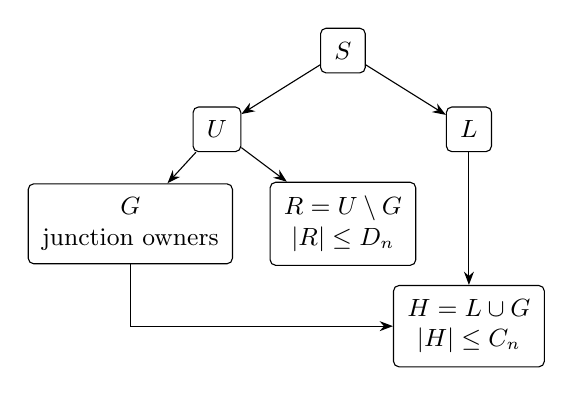
\begin{tikzpicture}[>=Stealth, every node/.style={font=\small},
 box/.style={draw,rounded corners=2pt,inner sep=5pt,align=center}]
 \node[box] (S) at (0,2.2) {$S$};
 \node[box] (U) at (-1.6,1.2) {$U$};
 \node[box] (L) at (1.6,1.2) {$L$};
 \node[box] (G) at (-2.7,0) {$G$\\junction owners};
 \node[box] (R) at (0,0) {$R=U\setminus G$\\$|R|\le D_n$};
 \node[box] (H) at (1.6,-1.3) {$H=L\cup G$\\$|H|\le C_n$};
 \draw[->] (S)--(U); \draw[->] (S)--(L);
 \draw[->] (U)--(G); \draw[->] (U)--(R);
 \draw[->] (L)--(H); \draw[->] (G.south)|-(H.west);
\end{tikzpicture}
\caption{The residual partition. First $S=U\sqcup L$, then
$U=G\sqcup R$. Transferring $G$ to the balanced part gives
$S=H\sqcup R$. Membership in $G$ uses witnesses inside $U$.}
\label{fig:partition}
\end{figure}

\begin{theorem}[Residual transfer]\label{thm:transfer}
For $n\ge6$, $Q_n\le C_n+D_n$ and consequently
$\ES(n)\le C_n+D_n+2$.
\end{theorem}
\begin{proof}
Let $S$ avoid an $(n-1)$-cap and a convex $n$-gon. The case $|S|\le1$
is immediate. At each point $x$, let $p(x)$ be the point minimizing
the slope of the incident unoriented line. The minimizer is unique
by general position. Partition $S$ into
\[
 U=\set{x:p(x)>x},\qquad L=\set{x:p(x)<x}.
\]
The map $p$ takes $U$ into $L$ and $L$ into $U$. For example, if
$x<y=p(x)<z=p(y)$, then $m(y,z)<m(x,y)$, and the weighted-average
identity gives $m(x,z)<m(x,y)$, a contradiction. The reversed argument
handles the other direction. A cap ending in $U$ extends to its chosen
right neighbor in $L$; a cup starting in $L$ extends to its chosen
left neighbor in $U$. Thus $U$ has no $(n-2)$-cap and $L$ has no
$(n-1)$-cup.

Let $G\subseteq U$ be the points ending an $(n-2)$-cup and starting
an $(n-3)$-cap, both in $U$. Put $H=L\cup G$ and $R=U\setminus G$.
The set $R$ satisfies the definition of $D_n$, since any forbidden
junction inside $R$ would also occur in $U$.

Suppose that $H$ contains an $(n-1)$-cup with endpoints $s,t$. If
$s\in L$, extend it left to an $n$-cup. If $t\in G$, extend its
$(n-3)$-cap in $U$ once into $L$, giving an $(n-2)$-cap starting at
$t$. At its junction with the supposed cup, one orientation yields
an $n$-cup and the other an $(n-1)$-cap. Hence $s\in G$ and $t\in L$.
Take the actual $(n-2)$-cup in $U$ ending at $s$ and extend its actual
outgoing $(n-3)$-cap once into $L$. The second point $q$ of this cap
lies in its original cap in $U$; extending that cap only appends its
last point. Therefore $q\ne t$.
\Cref{lem:threechain} applies and gives a contradiction. Hence $H$
has no $(n-1)$-cup, and inherits the other avoidances, so $|H|\le C_n$.
Now $S=H\sqcup R$ gives the result. The threshold statement follows
from \cref{prop:shift}.
\end{proof}

\section{The heptagon residual has a five-point transversal}\label{sec:deletion}
Write $B=M_7(5,6)$. Call a point a \emph{right root} if it starts no
three-cap in the specified ambient set. Every triple starting at a
right root is a cup, so it can be prepended to any cup to its right.

\begin{lemma}[Endpoint shift]\label{lem:root}
Every endpoint of a six-cup in a set counted by $D_7$ is a right root.
\end{lemma}
\begin{proof}
Let a six-cup end with $u,s$ and suppose $(s,q,r)$ is a three-cap.
If $(u,s,q)$ is a cup, append $q$ to obtain a seven-cup. Otherwise
$u$ ends the five-point prefix of the six-cup and starts the four-cap
$(u,s,q,r)$, a forbidden junction. Both possibilities are impossible.
\end{proof}

\begin{lemma}[Anchoring]\label{lem:anchor}
In a heptagon-free set, suppose $(a,b,t_3,t_4,t_5,t_6)$ is a six-cup
and $a$ is a right root. Every six-cup ending at $b$ starts at $a$.
\end{lemma}
\begin{proof}
If a start $x<a$ existed, $(x,a,b)$ would have to be a cap, since
otherwise $x$ could be prepended to the displayed cup. That cap and
the six-cup from $x$ to $b$ would form a heptagon. If $x>a$, the
right root $a$ could be prepended to the six-cup from $x$ to $b$.
Only $x=a$ remains.
\end{proof}

\begin{theorem}[Five-point deletion]\label{thm:deletion}
Every set counted by $D_7$ has a subset of at most five points meeting
every six-cup. In particular $D_7\le B+5$.
\end{theorem}
\begin{proof}
Let $E$ be all actual six-cup endpoints. By \cref{lem:root}, every
triple in $E$ is a cup; thus $|E|\le6$. If $|E|\le5$, delete $E$.
Otherwise write $E=(e_1,\ldots,e_6)$. This is a six-cup, and
\cref{lem:anchor} says that every six-cup ending at $e_2$ starts at
$e_1$. Delete $E\setminus\set{e_2}$. A surviving six-cup would have
an original endpoint in $E$, hence endpoint $e_2$, but would have to
start at the deleted point $e_1$. This is impossible.
The remaining set has no five-cap, six-cup, or heptagon, and has size
at most $B$.
\end{proof}

\section{Finite states and the balanced heptagon exclusion}\label{sec:balanced}
Down-set encodings of monotone paths are classical~\cite{MS,BB}.

The certificate conventions in this section use \emph{cup first, cap
second}. This differs from the order of the arguments of $M_n(a,b)$.
For reference, the two stored conventions are
\begin{center}
\begin{tabular}{ll}
\toprule
Certificate & Coordinates of a cell\\
\midrule
Section~\ref{sec:balanced}: heptagon & (cup, cap)\\
Sections~\ref{sec:octagons}--\ref{sec:319}: octagon & (cap, cup)\\
\bottomrule
\end{tabular}
\end{center}
For $u<v$, let $d(u,v)=(r(u,v),b(u,v))$, where $r+1$ and $b+1$ are
the longest cup and cap lengths ending at the exact pair $(u,v)$.
Define
\begin{equation}\label{eq:states}
 F(v)=\down\set{d(u,v):u<v}.
\end{equation}
All these ranks are actual maxima in the stated ambient set.

\begin{lemma}[Difference and chronology]\label{lem:difference}
For $u<v$, $d(u,v)\in F(v)\setminus F(u)$. Consequently states are
injective, and strict inclusion of two occupied states forces the same
order on their owners.
\end{lemma}
\begin{proof}
If $d(u,v)\in F(u)$, some actual predecessor $t<u$ has
$d(t,u)\ge d(u,v)$ coordinatewise. According to the orientation of
$(t,u,v)$, extending an attaining cup or cap contradicts one of the
two maxima at $(u,v)$. Thus the difference is nonempty. Equal states,
or an earlier state containing a later one, would contradict this
conclusion.
\end{proof}

With no $a$-cap or $b$-cup, the states lie in $[b-2]\times[a-2]$,
whose number of down-sets is $\binom{a+b-4}{a-2}$, including the empty
state. A Ferrers tuple denotes column heights, with trailing zeros
where required by the data format. The finite models permit every
chronological order compatible with inclusion; they do not sort
incomparable states into a preferred order.

\begin{theorem}[A sharp ETV case; computer-assisted]\label{lem:B25}
Every set of 26 points in $\mathbb R^2$, in general position and with
distinct $x$-coordinates, contains a five-cap, a six-cup, or seven
points in convex position. There is a 25-point set avoiding all three.
Thus $M_7(5,6)=25$; reflection also gives $M_7(6,5)=25$.
\end{theorem}
\begin{proof}[Certificate reduction]
For the lower bound, the Erd\H{o}s--Szekeres construction~\cite{ES61},
in the restricted form of Erd\H{o}s--Tuza--Valtr~\cite{ETV}, gives
$\sum_{i=1}^{3}\binom5i=25$ points with none of the three configurations;
see also Baek--Balko~\cite[Section~4]{BB}.
The archive also contains an exact rational 25-point witness and a
separate integer checker confirming maximum cup length five, maximum
cap length four, and no convex heptagon among all
$\binom{25}{7}=480\,700$ seven-point subsets.
This lower-bound check is separate from the Lean upper-bound theorem.

A hypothetical 26-point counterexample has 26 distinct actual states
in $[4]\times[3]$, a universe of 35 states, and hence nine missing
states. The empty state and the one-cell state occur at the first two
points; the third has one of the two two-cell states. In the certificate's
area-sorted dictionary, an eligible hole set therefore avoids indices
0 and 1 and does not contain both 2 and 3. There are exactly
\[
 \binom{33}{9}-\binom{31}{7}=35\,937\,525
\]
eligible hole sets.

The certificate derives necessary hole clauses from pair-label
differences, exact corner attainment, shared predecessor witnesses, actual
owner order, four-point sign constraints, and common-endpoint paths.
A five-cup and four-cap with common endpoints give a heptagon, so
excluding just this type is a necessary restriction. The Lean coverage stage refutes a CNF consisting of 91,720 derived
hole clauses, a cardinality encoding, and one padding tautology:
461 variables and 93,169 clauses in total. Its LRAT proof has
381,647 additions. Separately, two enumerations, recursive and
fixed-popcount, verify that none of the eligible hole sets survives.
\Cref{app:restricted} describes the primitive semantics and proof format.
\end{proof}

Consider now a balanced avoiding set $S$ of size 50. Let $\cupS$ and
$\capS$ be its actual five-cup and five-cap starters, and $\cupE$ and
$\capE$ the corresponding endpoint sets.

\begin{lemma}[Equality partition]\label{lem:equality}
There is an integer $t$ such that
\[
 S=\cupS\sqcup\capE=\capS\sqcup\cupE,
 \qquad |\cupS|=|\capS|=|\cupE|=|\capE|=25,
\]
and, with
\[
 L=\cupS\cap\capS,\quad X=\cupS\cap\cupE,
 \quad Y=\capS\cap\capE,\quad R=\cupE\cap\capE,
\]
one has $|X|=|Y|=t$ and $|L|=|R|=25-t$.
\end{lemma}
\begin{proof}
The set $\cupS$ contains no five-cap: joining the end of such a cap
to an actual outgoing five-cup extends one of them to a six-chain.
Its complement contains no five-cup. By \cref{lem:B25} and reflection,
both parts have size at most 25, and hence exactly 25. Color exchange
and order reversal give the same endpoint counts. A point ending a
five-cap cannot start a five-cup, by the same junction argument, so
the disjoint pairs each exhaust $S$. Taking their four intersections
gives the stated cardinalities.
\end{proof}

\begin{lemma}[Population certificates]\label{lem:populations}
In a planar set with no six-cup, six-cap, or heptagon:
\begin{enumerate}[label=(\roman*)]
\item at most thirteen points both end and start five-cups;
\item any subset avoiding five-cups and five-caps, whose last point
starts a five-cup in the ambient set, has at most nineteen points;
\item if $N_0$ consists of points ending neither five-chain and $N_2$
of points ending both, then
\[\min(|N_0|,|N_2|)\le16.\]
\end{enumerate}
\end{lemma}
\begin{proof}[Necessary reductions and finite certificates]
For (i), select fourteen supposed through-cup points, a five-cup ending
at the first, and a five-cup starting at the last. Exactly 22 points
are selected: fourteen core points and four on each side. Any core
four-cap extends at both ends to a six-cap, so the core has cap length
at most three. Its cap paths extend by one at each end, whereas its
cup paths remain valid ambient paths. The source records exact core
recurrences and these valid implications for ambient ranks, without
requiring ambient attainment in the selection. Its refutation has
3,009 additions.

For (ii), select a supposed 20-point core and the four other vertices
of an actual five-cup from its last point. Incoming ranks ending in
the core are recomputed there; neither color reaches five. The resulting
24-point source is refuted in 79,173 additions.

For (iii), the incoming states of $N_0$ are the twenty ideals of
$[3]^2$. Those of $N_2$ are the twenty ideals
$(4,1+h_1,1+h_2,1+h_3)$ with $h$ an ideal of $[3]^2$. Select seventeen
owners from each family, retaining the ambient first two points.
A named-owner source permits all such selections and all their
inclusion-compatible orders. Pair ranks are ambient and paths are
selected. Its refutation has 102,563 additions.

All three formulas include the necessary four-point packet constraints
and common-endpoint polygon exclusions. The compact formulas and refutations are embedded in the Lean sources.
Their geometric interpretations and logical soundness are proved there;
\cref{sec:formal,app:cnf} describes the interface. Thus each
supposed configuration supplies an assignment to a refuted formula.
\end{proof}

\begin{corollary}\label{cor:range}
In \cref{lem:equality}, $9\le t\le13$. Every twenty ambient five-cup
starters contain an internal five-cup, and a 25-point starter class
has at least six actual internal five-cup sources.
\end{corollary}
\begin{proof}
The through-cup bound gives $t\le13$. In the equality partition,
$N_0=L$ and $N_2=R$, so $25-t\le16$ and $t\ge9$.
Any set of twenty cup starters has no internal five-cap by the
junction argument. If it had no five-cup either, part (ii) of
\cref{lem:populations}, applied to its last point, would be contradicted.
Finally, deleting at most five internal sources from a 25-point starter
class would leave at least twenty ambient starters with no internal
five-cup. Deletion cannot create a new path, so at least six sources
must exist.
\end{proof}

\begin{proposition}[Balanced heptagon bound]\label{prop:balanced}
$C_7\le49$.
\end{proposition}
\begin{proof}
Assume $|S|=50$ and let $K=\cupS$. Retain the 25 points of $K$ and
the four other points of an actual five-cup from $\max K$. For a point
of $K$, no ambient five-cap can end there, so its actual incoming
state lies in the 35-state universe $[4]\times[3]$. Fifteen of these
states have width four; their active population is precisely $t$.
The low-width owners are also cap starters by \cref{lem:equality}.
All 25 states are actual ambient states, not states recomputed after
selecting these 29 points.

Reflect the whole configuration if necessary to make its first triple
a cup, and select the corresponding starter class anew. The four
possible initial packets, in order $012,013,023,123$, are
$1000,1100,1110,1111$. A cup and cap share at most two vertices.
The initial three-cup therefore forces the first five ambient points
to have no ending five-cap, and hence to belong to $K$. In the $1111$
sector the first six points similarly belong to $K$. Exhaustive
literal enumeration retains all seven five-point extensions of $1000$
and all 118 six-point extensions of $1111$ without a six-cup.
The $1100$ and $1110$ sectors remain in the primary formula until
their exclusions are derived.

The primary formula has 151,801 variables and 4,017,399 clauses. It includes \cref{cor:range}, the six-source condition,
free order for incomparable owners, shared ambient pair labels,
selected paths, exact core outgoing paths, and the prefix alternatives.
Exact incoming attainment is imposed only at retained ambient prefix
points, where every predecessor is present. The variable meanings
and necessary clause families are listed in Appendix~\ref{app:cnf}.

A single proof over this unaugmented primary formula derives the empty
clause. It contains 1,989,465 additions and 84,721,022 ordered hints.
Its derivation includes the exclusions of $t=13,9,12$, the two mixed
prefixes, and both final cases $t=10,11$. These case facts are derived
within the proof; the final contradiction has no case assumption.
The compact source uses 190,932 indexed clauses of the primary formula;
the same number of proof additions suffices. Checked replay of
this compact proof establishes unsatisfiability. The formal proof additionally checks each retained clause against a
proved necessary schema under one common assignment.

Every supposed planar $S$ supplies a truthful assignment to the
retained source, so unsatisfiability is a contradiction. Any larger
avoiding set would contain an avoiding fifty-point subset.
\end{proof}

Combining \cref{lem:B25,thm:deletion,prop:balanced,thm:transfer} gives
\[
 \ES(7)\le49+(25+5)+2=81.
\]
The classical construction~\cite{ES61} supplies the lower endpoint
$\ES(7)\ge33$; it is separate from the formalized upper bound.

\input{octagons}
\section{Formalization and reproducibility}\label{sec:formal}\label{sec:certificates}
The two final declarations are
\begin{center}
\code{ES7FinalVerified.es7\_le\_81},\qquad
\code{ES8Final.es8\_le\_319}.
\end{center}
Appendix~\ref{app:statements} prints their types and the definitions
of general and convex position, together with the exact axiom output.
The companion module \code{StatementAudit.lean} proves that
\code{ConvexPosition} is equivalent to mathlib's
\code{ConvexIndependent} for the inclusion of the point set, and
restates both bounds with that standard predicate. It adds no
native-evaluation dependency.

Each theorem quantifies over a finite subset of $\mathbb R^2$. General position
requires nonzero oriented area for every distinct triple; the conclusion
is a subset of cardinality seven or eight, each of whose points lies
outside the convex hull of the others. The statements have no additional
numerical or geometric hypotheses. The geometric reductions are formalized for $n=7$ and $n=8$.
The classical lower constructions in \cref{thm:main} are cited
separately, not claimed as formalized here.

\subsection{The proof boundary}
There are three distinct obligations. First, geometric necessity sends
every hypothetical planar counterexample to one assignment satisfying
the finite source. Second, a general checker-soundness theorem turns
acceptance of a certificate into a contradiction for that source.
Third, the concrete checker accepts the supplied finite data.
The first two are ordinary Lean proofs. The third uses
\code{native\_decide} for the large certificates and finite catalogues.
The five final heptagon refutations use Lean's standard-library
\code{Std.Tactic.BVDecide.LRAT} checker and its \code{check\_sound}
theorem. The earlier restricted primitive-replay stage has its own
proved RUP layer. No SAT solver or numerical optimizer is trusted to
assert unsatisfiability.

The standard axioms in both final dependency lists are
\begin{center}
\code{propext}, \code{Classical.choice}, \code{Quot.sound}.
\end{center}
The heptagon theorem additionally uses 19 native-evaluation checks,
and the octagon theorem uses eight. There is no \code{sorryAx} and no
additional mathematical axiom. Native evaluation additionally trusts
Lean's compilation and execution infrastructure; this is not a
kernel-only evaluation of every finite computation. Exact axiom names,
source hashes, and the toolchain are recorded in the archive.
The 208 bundled project modules contain no occurrence of
\code{implemented\_by}, \code{extern}, \code{csimp}, or \code{unsafe}.
This is a scoped source check, not an absence claim for the transitive
runtime: Lean's standard array operations, for example, have external
implementations. The compiler, its rewrites, and runtime remain
within the stated native-evaluation trust boundary.

For the heptagon closure, the source decoder checks all 190,932 retained
clauses against proved schemas. One normalized configuration supplies
the state owners, the common chronological order, all actual ambient
ranks, the induced-core ranks, and one shared terminal five-cup.
A source classifier proposes schema identifications but is untrusted:
Lean checks literal decoding, clause equality, schema validity, and
complete coverage before applying the refutation.

For octagons, both omission trees and all their capacity rows are
connected to the same geometric occupancy assignment. In particular,
the 973 historically transported residual supports now have direct
cyclic proofs. The block rows use an audited port of Baek's own Lean
formalization, with its Apache-2.0 attribution retained. The port's
combinatorial boundary predicate is connected to the real-plane
convex-hull predicate by an explicit theorem.

\subsection{Lessons from formalization}
The completed proofs make three distinctions especially useful for
further computations.

\emph{Actual and inherited ranks.} A longest-path value has an attaining
witness in a specified set. Restriction can destroy that witness.
The heptagon proof therefore recomputes core recurrences, while keeping
ambient ranks separately. The octagon proof deliberately uses the
weaker admissible-label interface, which is hereditary and requires no
new attainment after transport.

\emph{Local validity and shared existence.} Individually feasible
witnesses need not coexist. The heptagon source uses one interpretation
of every owner, sign, order, and path flag. Prefix coverage is proved
before exclusions are applied; no preferred order of incomparable
states is imposed. In the octagon proof, triplewise cyclic certification
survives missing endpoints and therefore justifies multi-omission rows.

\emph{Projective geometry and cardinality.} The formal projective map
is applied only on a positive-denominator chart. Convex combinations
are transported with renormalized positive weights, not unchanged
affine coefficients. A finite-exception shear first separates
abscissae, sorting is bijective, and the deleted root is treated
separately. The three-chain exception $q\ne t$ is discharged by actual
membership in the two parts of the partition. These steps establish
both the ordinary planar meaning and the two-point adjustment.

\subsection{Finite data and reconstruction}
The heptagon refutations use reverse unit propagation: assuming the
negation of a proposed clause, the listed earlier clauses must force a
conflict. Soundness and the final empty clause are checked in Lean.
The main proof sizes are shown below; the restricted-25 certificate
has its own primitive, replay, and coverage stages.
\begin{center}
\small
\begin{tabular}{lrr}
\toprule
Obligation & Retained source clauses & Proof additions\\
\midrule
Restricted hole coverage & 93,169 & 381,647\\
Through-cup population $\le13$ & 5,077 & 3,009\\
Terminal core $\le19$ & 25,074 & 79,173\\
Joint endpoint population & 59,479 & 102,563\\
Balanced fifty-point exclusion & 190,932 & 1,989,465\\
\bottomrule
\end{tabular}
\end{center}
The coverage formula has 461 variables.
The octagon certificates have the following sizes. Each branch covers
both Boolean values, and every weighted leaf has a strict integer
contradiction in its own context.
\begin{center}
\small
\begin{tabular}{lrrrr}
\toprule
Obligation & States & Rows & Branches & Leaves\\
\midrule
Balanced bound $193$ & 252 & 2,685 & 1,590 & 1,591\\
Residual bound $124$ & 154 & 1,187 & 7,314 & 7,315\\
\bottomrule
\end{tabular}
\end{center}
The archive contains 208 project modules, including embedded certificates
and the Baek port. It pins Lean 4.32.0-rc1 and a specific mathlib commit.
The complete library was rebuilt from source without precompiled
project modules in 1,290 seconds on an ARM64 macOS host; peak memory
was not recorded. This release preserves those proof sources byte for
byte and includes a separately compiled statement-equivalence and
parser-guard module. The latter proves that a nonempty numeric source row cannot
parse as an empty clause; all five literal sources pass the independent
check of that premise.
The accompanying audit distinguishes the full build from later
source-identical extraction checks. From the archive root, with the pinned
mathlib checkout and its dependencies already built, run
\begin{verbatim}
python3 tools/verify_release.py --mathlib /path/to/mathlib
\end{verbatim}
This verifies file identities, rebuilds the project in a fresh directory,
and checks both final declarations and their exact allowed axiom lists.
The archive README gives the dependency setup and PDF build commands.
Certificate discovery is not needed for replay. Independent checks are
\begin{verbatim}
python3 tools/check_octagon_finite.py
python3 tools/check_heptagon_replays.py
python3 tools/check_examples_and_counts.py
python3 tools/check_residual_lower.py
\end{verbatim}
The first command reconstructs both octagon state universes and all
directed differences, certifies all 3,849 cyclic families and 23 block
maps, compares the JSON and Lean data, and replays all 8,906 leaves
with complete branch coverage. This finite audit runs without Lean or
native evaluation; it uses the geometric lemmas proved above. It is
an independent executable check, not a change to the Lean theorem's
dependency list.

The second command compiles a separate C++ RUP checker. All four
population/closure proofs pass unchanged. The coverage proof contains
one satisfied, redundant hint (473786 in step 473998); the command
reproduces its strict rejection and then replays with exactly that
hint omitted. All clauses and other hints remain unchanged, as do the
sealed Lean files. The final coverage replay has 381,647 additions;
the closure replay has 1,989,465. This checker is not itself formally
verified. A replay through an external verified LRAT implementation
and a second-platform full build remain further audits.
The third command checks the ten-state example, exact 25-point control,
and comparison arithmetic. The fourth checks the full residual predicate
and every seven-point subset of the 26-point lower example in Section~9.
The capacity, strict-replay, and residual-control checkers include rejection controls.

\Needspace{12\baselineskip}
\subsection{Archive identification}
The companion bundle is
\begin{center}\code{es7\_es8\_bounds\_81\_319\_v1.zip}.\end{center}
The SHA-256 below identifies the unchanged formal manifest.
Its path in the bundle is
\begin{center}\code{formal/MANIFEST.json}.\end{center}
\begin{center}\small\ttfamily
\input{formal_manifest_hash}
\end{center}
The bundle includes the complete paper sources, proof sources,
certificates, checker commands, and hash manifest. The paper and companion archive share the DOI
\href{https://doi.org/10.5281/zenodo.22842891}{10.5281/zenodo.22842891}.

\section{Further directions}
Either $D_7\le29$ or $C_7\le48$ would give $\ES(7)\le80$.
There are, however, unconditional limits to improving the two capacities
separately. The classical restricted constructions~\cite{ES61,ETV} give
$C_7\ge30$, $C_8\ge62$, and $M_8(6,6)\ge50$. A set counted by
$M_8(6,6)$ has no six-cup, hence no residual junction, so $D_8\ge50$.
The archive also supplies an exact 26-point residual set. Its five-cup
endpoints and four-cap starting points are disjoint; the checker verifies
this condition and excludes a heptagon in all
$\binom{26}{7}=657\,800$ seven-point subsets. Thus $D_7\ge26$.
Consequently,
\[
 C_7+D_7+2\ge58,\qquad C_8+D_8+2\ge114.
\]
These are floors of the independently optimized additive bound
\eqref{eq:bridge}, not lower bounds on $\ES(7)$ or $\ES(8)$.
Of the 48-point gap from 81 to the conjectural 33, at most
$81-58=23$ points can be recovered by improving the separate capacities;
at least $58-33=25$ require their joint compatibility or another argument.

The conjecture of Erd\H{o}s, Tuza, and Valtr would give:
\begin{center}
\begin{tabular}{lccc}
\toprule
Quantity & Known lower bound & Proved upper bound & Under ETV\\
\midrule
$C_7$ & $\ge30$ & $\le49$ & $=30$\\
$D_7$ & $\ge26$ & $\le30$ & $=26$\\
$C_8$ & $\ge62$ & $\le193$ & $=62$\\
$D_8$ & $\ge50$ & $\le124$ & $\le57$\\
\bottomrule
\end{tabular}
\end{center}
Its proposed value for $M_n(a,b)$ is
$\sum_{i=n-b}^{a-2}\binom{n-2}{i}$~\cite{ETV,Baek}.
For residual upper bounds we use $D_n\le M_n(n-2,n)$;
the equality for $D_7$ additionally uses the checked lower example.
Thus ETV would make $C_7+D_7+2=58$ and place
$C_8+D_8+2$ in $[114,121]$. The latter interval is conditional;
only its lower endpoint is established unconditionally here.

The additive bound discards compatibility between the two parts. Retaining
their shared witnesses, or bounding the asymmetric class $Q_n$ directly,
may overcome these limits. For octagons, admissible state differences
also offer a way to certify further hereditary capacities. These are
open tasks; no incomplete search enters the results above.

\subsection*{Acknowledgments}
{\raggedright
This work benefited from research assistance by \mbox{OpenAI's} AI systems, including proof exploration, exact computational checks, and manuscript preparation. All responsibility for the content and conclusions of this work rests with the author.\par}

\subsection*{Licence}
The manuscript, original exposition, and original accompanying certificate
data are licensed under the Creative Commons Attribution 4.0 International
licence (CC BY 4.0). Original program code, including the original Lean
formalization and verification scripts, is licensed under the MIT licence.
The attributed port of Jineon Baek's \emph{ErdosTuzaValtr} formalization
retains its Apache-2.0 licence. Other third-party material and external
dependencies retain their respective licences. The accompanying archive
contains the applicable licence information and attribution notices.

\appendix
\input{source_semantics}
\input{statement_audit}
\clearpage
\begin{thebibliography}{99}
\raggedright
\bibitem{Baek} J. Baek,
On the Erd\H{o}s--Tuza--Valtr conjecture,
\emph{European Journal of Combinatorics} \textbf{124} (2025), 104085.
\href{https://doi.org/10.1016/j.ejc.2024.104085}{doi:10.1016/j.ejc.2024.104085}.

\bibitem{BB} J. Baek and M. Balko,
The Erd\H{o}s--Szekeres conjecture revisited,
\emph{Journal of Combinatorial Theory, Series A} \textbf{222} (2026), 106195.
\href{https://doi.org/10.1016/j.jcta.2026.106195}{doi:10.1016/j.jcta.2026.106195}.
Conference version: SoCG 2025, LIPIcs 332, 13:1--13:15.

\bibitem{BV} M. Balko and P. Valtr,
A SAT attack on the Erd\H{o}s--Szekeres conjecture,
\emph{European Journal of Combinatorics} \textbf{66} (2017), 13--23.
\href{https://doi.org/10.1016/j.ejc.2017.06.010}{doi:10.1016/j.ejc.2017.06.010}.

\bibitem{DDSZ} G. Dam\'asdi, Z. Dong, M. Scheucher, and J. Zeng,
Saturation results around the Erd\H{o}s--Szekeres problem,
\emph{European Journal of Combinatorics} \textbf{131} (2026), 104236.
\href{https://doi.org/10.1016/j.ejc.2025.104236}{doi:10.1016/j.ejc.2025.104236}.

\bibitem{Dumitru} B. Dumitru,
Notes on the 33-point Erd\H{o}s--Szekeres problem,
\href{https://arxiv.org/abs/2512.24061}{arXiv:2512.24061v1} (2025).

\bibitem{ES35} P. Erd\H{o}s and G. Szekeres,
A combinatorial problem in geometry,
\emph{Compositio Mathematica} \textbf{2} (1935), 463--470.

\bibitem{ES61} P. Erd\H{o}s and G. Szekeres,
On some extremum problems in elementary geometry,
\emph{Ann. Univ. Sci. Budapest. E\"otv\"os Sect. Math.}
\textbf{3--4} (1960--1961), 53--62.

\bibitem{ETV} P. Erd\H{o}s, Z. Tuza, and P. Valtr,
Ramsey-remainder,
\emph{European Journal of Combinatorics} \textbf{17} (1996), 519--532.
\href{https://doi.org/10.1006/eujc.1996.0045}{doi:10.1006/eujc.1996.0045}.

\bibitem{HMPT} A. F. Holmsen, H. Nassajian Mojarrad, J. Pach, and G. Tardos,
Two extensions of the Erd\H{o}s--Szekeres problem,
\emph{Journal of the European Mathematical Society} \textbf{22} (2020), 3981--3995.
\href{https://arxiv.org/abs/1710.11415}{arXiv:1710.11415}.

\bibitem{KK} V. Koshelev and A. Koshka,
Combinatorial geometry of Erd\H{o}s--Szekeres type problems:
SAT/ASP modeling and linear subreduction,
\href{https://arxiv.org/abs/2604.20120}{arXiv:2604.20120v1} (2026).

\bibitem{Maric} F. Mari\'c,
Fast formal proof of the Erd\H{o}s--Szekeres conjecture for convex polygons
with at most 6 points, \emph{Journal of Automated Reasoning}
\textbf{62} (2019), 301--329.
\href{https://doi.org/10.1007/s10817-017-9423-7}{doi:10.1007/s10817-017-9423-7}.

\bibitem{MS} G. Moshkovitz and A. Shapira,
Ramsey theory, integer partitions and a new proof of the
Erd\H{o}s--Szekeres theorem,
\emph{Advances in Mathematics} \textbf{262} (2014), 1107--1129.

\bibitem{MV} H. Nassajian Mojarrad and G. Vlachos,
An improved upper bound for the Erd\H{o}s--Szekeres conjecture,
\emph{Discrete \& Computational Geometry} \textbf{56} (2016), 165--180.
\href{https://doi.org/10.1007/s00454-016-9791-5}{doi:10.1007/s00454-016-9791-5}.

\bibitem{NY} S. Norin and Y. Yuditsky,
Erd\H{o}s--Szekeres without induction,
\emph{Discrete \& Computational Geometry} \textbf{55} (2016), 963--971.
\href{https://arxiv.org/abs/1509.03332}{arXiv:1509.03332}.

\bibitem{EmptyLean} B. Subercaseaux, W. Nawrocki, J. Gallicchio,
C. Codel, M. Carneiro, and M. J. H. Heule,
Formal verification of the empty hexagon number,
in \emph{ITP 2024}, LIPIcs \textbf{309} (2024), 35:1--35:19.
\href{https://doi.org/10.4230/LIPIcs.ITP.2024.35}{doi:10.4230/LIPIcs.ITP.2024.35}.

\bibitem{Suk} A. Suk,
On the Erd\H{o}s--Szekeres convex polygon problem,
\emph{Journal of the American Mathematical Society} \textbf{30} (2017), 1047--1053.
\href{https://arxiv.org/abs/1604.08657}{arXiv:1604.08657}.

\bibitem{SP} G. Szekeres and L. Peters,
Computer solution to the 17-point Erd\H{o}s--Szekeres problem,
\emph{ANZIAM Journal} \textbf{48} (2006), 151--164.
\href{https://doi.org/10.1017/S144618110000300X}{doi:10.1017/S144618110000300X}.

\bibitem{TV98} G. T\'oth and P. Valtr,
Note on the Erd\H{o}s--Szekeres theorem,
\emph{Discrete \& Computational Geometry} \textbf{19} (1998), 457--459.
\href{https://doi.org/10.1007/PL00009363}{doi:10.1007/PL00009363}.

\bibitem{TV05} G. T\'oth and P. Valtr,
The Erd\H{o}s--Szekeres theorem: upper bounds and related results,
in \emph{Combinatorial and Computational Geometry}, MSRI Publications
\textbf{52}, Cambridge University Press, 2005, 557--568.
\end{thebibliography}

\end{document}
